\documentclass[border=2mm]{standalone}
\usepackage{tikz}
\tikzset{
    vertex/.style = {
        circle,
        draw,
        fill=black!20,
        outer sep = 3pt,
        inner sep = 3pt,
    },
    edge/.style = {->,> = latex'}
}
\begin{document}

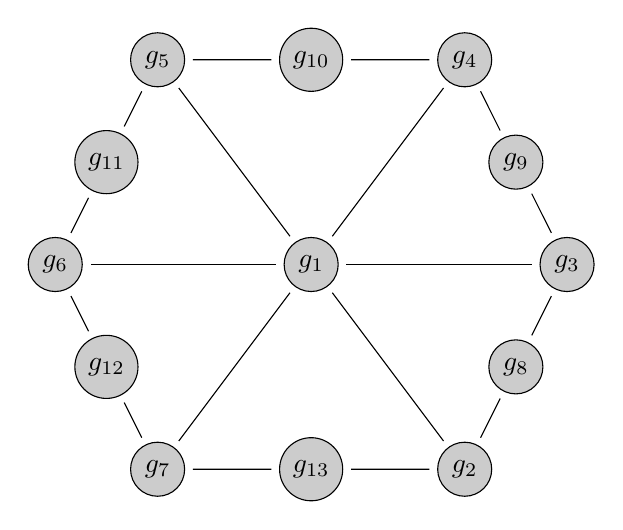
\begin{tikzpicture}[scale=1.3, auto=center]
  
  % Define all vertices using the consistent 'vertex' style
  \node[vertex] (a1)  at (0,0)     {$g_1$};
  \node[vertex] (a2)  at (1.5,-2)  {$g_2$};
  \node[vertex] (a3)  at (2.5,0)   {$g_3$};
  \node[vertex] (a4)  at (1.5,2)   {$g_4$};
  \node[vertex] (a5)  at (-1.5,2)  {$g_5$};
  \node[vertex] (a6)  at (-2.5,0)  {$g_6$};
  \node[vertex] (a7)  at (-1.5,-2) {$g_7$};
  \node[vertex] (a8)  at (2,-1)    {$g_8$};
  \node[vertex] (a9)  at (2,1)     {$g_9$};
  \node[vertex] (a10) at (0,2)     {$g_{10}$};
  \node[vertex] (a11) at (-2,1)    {$g_{11}$};
  \node[vertex] (a12) at (-2,-1)   {$g_{12}$};
  \node[vertex] (a13) at (0,-2)    {$g_{13}$};
  
  % Draw undirected edges (as per original -- commands)
  % Central connections from a1
  \draw (a1) -- (a2);
  \draw (a1) -- (a3);
  \draw (a1) -- (a4);
  \draw (a1) -- (a5);
  \draw (a1) -- (a6);
  \draw (a1) -- (a7);
  
  % Connections from a2
  \draw (a2) -- (a8);
  \draw (a2) -- (a13);
  
  % Connections from a3
  \draw (a3) -- (a8);
  \draw (a3) -- (a9);
  
  % Connections from a4
  \draw (a4) -- (a9);
  \draw (a4) -- (a10);
  
  % Connections from a5
  \draw (a5) -- (a10);
  \draw (a5) -- (a11);
  
  % Connections from a6
  \draw (a6) -- (a11);
  \draw (a6) -- (a12);
  
  % Connections from a7
  \draw (a7) -- (a12);
  \draw (a7) -- (a13);
  
\end{tikzpicture}

\end{document}
